\chapter{COMPUTING CONNECTED MATCHINGS}

While the extremal problem of connected matchings has driven most of the theoretical development to date, there is another aspect of connected matchings that demands our attention.  How do we {\it find} large connected matchings in graphs?  In particular, how do we compute the size of the largest connected matching in a particular graph?  Plummer et. al show in \cite{PST} that this problem is NP-hard in general.

A connected matching of size $k$ has a clique minor of size $k$, so it may not be surprising that the general problem of finding connected matchings is difficult.  There is a ``clique-like'' element to the problem, and so we might expect that the computational difficulty is similar to clique problems.  However, maximum matchings in graphs can be found efficiently.  Edmonds in \cite{edmonds} showed an algorithm that computes the maximum matching in a graph in time polynomial to the number of vertices in the graph.  Furthermore, there are many elegant matching algorithms that we may adapt to the problem of constructing a maximum connected matching.

In this chapter, we investigate computational problems concerning connected matchings in special families of graphs.  We attempt to utilize the special structure of these families to develop algorithms that find maximum connected matchings.

\section{Known results}

In \cite{K_Cam_conn_match}, Cameron shows that the maximum connected matching problem is solvable in polynomial time for {\it chordal} graphs,   
%
by considering connected matchings as matchings contained in {\it neighborly} sets of edges.  
%
Neighborly sets of edges from a graph $G$ correspond to cliques in the square of the line graph of $G$, $L(G)^2$.  
%
It then follows that if $L(G)^2$ has $M$ maximal cliques, then the maximum connected matching in $G$ can be found by solving $M$ maximum matching problems.  
%
Hence, we state the following general result from which the result on chordal graphs follows.
%
\bthm{If $\mathcal{P}$ is a class of graphs such that for any $G \in \mathcal{P}$ with $n$ vertices, the number of maximal cliques in $L(G)^2$ is less than $f(n)$ where $f$ is a polynomial, then the maximum connected matching problem can be solved in polynomial time for graphs from $\mathcal{P}$.}
%
The square of the line graph of a chordal graph is itself a chordal graph\footnote{In fact, Cameron showed in \cite{indmatch} that a larger class of graphs, the {\it weakly chordal} graphs also have this property.  That is, the square of the line graph of a weakly chordal graph is also weakly chordal.}, and hence has a polynomial number of maximal cliques. 
%

Conversely, Cameron also shows that the maximum weighted connected matching problem remains NP-complete on (0,1)-weighted bipartite graphs.  
%
It is not difficult to reduce this problem to the maximum clique problem on general graphs,  
%
by taking any graph $H$ and replacing each vertex $v$ with a new edge joining two new vertices $v_1$ and $v_2$, assigning the edge $v_1v_2$ a weight of 1.  
%
If two vertices $u$ and $v$ are adjacent in $H$, we produce edges $u_1v_2$ and $u_2v_1$ of weight zero.
%  
In the resulting graph, the edges of positive weight in any connected matching correspond to a clique in $H$ and vice versa.
%
It is important to note that this reasoning does not extend to the unweighted bipartite graphs.  



\section{Chordal bipartite graphs}

To extend the results in the previous section, we turn to a relaxation of chordal graphs, the {\it weakly} chordal graphs. 
%
A weakly chordal graph is a graph in which every cycle of length five or greater has a chord.  
%
Also, we closely examine those weakly chordal graphs that are also bipartite; these graphs are known as {\it chordal bipartite} graphs (see Figure \ref{inclusion}).  
\begin{figure}
	\begin{center}
		
\begin{tikzpicture}[thick,scale=0.4]


\draw[ fill = red, opacity = 0.25] (0,0) circle (3);
\draw[ fill = blue, opacity = 0.25, thin] (3.5,0) circle (3);
\draw[ fill = red, opacity = 0.25] (0,0) circle (1.5);

\draw  (-4,4.5) node[words]{weakly chordal}
	edge [->, thin] (-1,2.9);

\draw  (-4,-4.5) node[words]{chordal}
	edge [->, thin] (-1.3,-0.9);

\draw (1,-4.5) node[words]{acyclic};
\draw node[words] (1,-4) {}
	edge [->, thin] (1,-.5);


\draw (6, -5.5) node[words]{chordal bipartite}
	edge[->, thin] (2,-.5);
\draw (5, 4.5) node[words]{bipartite}
	edge[->,thin] (4.5,2.85);

\end{tikzpicture}

	\end{center}
	\label{inclusion}
	\caption{Inclusion diagram}
\end{figure}

An important characterization of chordal bipartite graphs is that any non-empty induced subgraph of a chordal bipartite graph contains a {\it bisimplicial edge}.  
%
An edge $uv$ is bisimplicial if the neighborhoods of the endpoints induce a complete bipartite graph.  
%
That is, for any $a\in N(u)$ and $b\in N(v)$, $ab$ is an edge of the graph.  
%
Bisimplicial edges equip the chordal bipartite graphs with a perfect edge without vertex elimination ordering, i.e., upon removing a bisimplicial edge from a chordal bipartite graph, the resulting graph is still chordal bipartite.  These results, among others developing the theory of chordal bipartite graphs, can be found in \cite{Gol_Goss}.

\subsection{Inert bisimplicial edges}
If a graph is non-separable, then we quickly compute the maximum connected matching using any maximum matching algorithm we choose.  
%
The following result of Golumbic \cite{Golumbic} is valuable when dealing with non-separable chordal bipartite graphs.
%
\bthm{ Let $H$ be a chordal bipartite graph.  If $H$ is separable, then it has at least two separable bisimplicial edges.}
%
We will see shortly that once we have identified a pair of bisimplicial edges, we can always remove one of them from the graph without reducing the size of a maximum connected matching in the graph.  
%

Let us say that an edge $e$ in a graph $G$  is {\it inert} if $\nu_c(G) = \nu_c(G-e)$.  
%
Bisimplicial edges in chordal bipartite graphs are inert unless the conditions in the following lemma are satisfied.
%
\blem{Let $G = (A, B; E)$ be chordal bipartite.  A bisimplicial edge $e = uv$ is inert unless at least one of the following is true: 
	\begin{enumerate}
 		\item $e$ is contained in every maximum connected matching.
		\item For any maximum connected matching $M$, every edge of $M$ has
 exactly one endpoint adjacent to an endpoint of $e$.
		\item For any maximum connected matching $M$, $N(e)$ is covered by M.
	\end{enumerate}\label{cbp_lemma}
}
%
\begin{figure}
	\begin{center}
	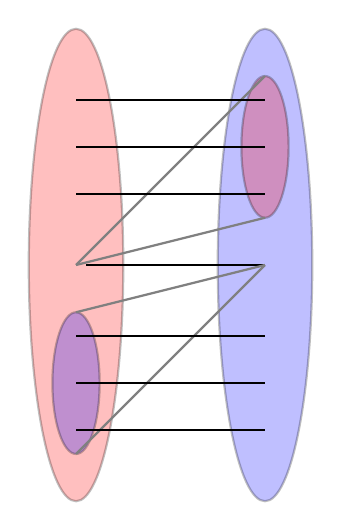
\begin{tikzpicture}[thick,scale=0.6]

\draw[fill = red, opacity = 0.25]  (-2,0) ellipse(1 and 5);
\draw [fill = blue, opacity = 0.25](-2,-2.5) ellipse (0.5 and 1.5);
\draw[fill = blue, opacity = 0.25] (2,0) ellipse (1 and 5);
\draw[fill = red, opacity = 0.25] (2,2.5) ellipse (0.5 and 1.5);
\draw (-2,0) node[]{}
	edge[] (2,0);
\draw (2,0) node[]{};

\draw[color = gray] (-2,0)--(2,4);
\draw[color = gray] (-2,0)--(2,1);
\draw[color = gray] (2,0)--(-2,-1);
\draw[color = gray] (2,0)--(-2,-4);

\draw (-2,3.5)--(2,3.5);
\draw (-2,2.5)--(2,2.5);
\draw (-2,1.5)--(2,1.5);
\draw (-2,-3.5)--(2,-3.5);
\draw (-2,-2.5)--(2,-2.5);
\draw (-2,-1.5)--(2,-1.5);
\end{tikzpicture}
	\end{center}
	\label{bisimp_pic}
	\caption{Picture of a non-inert bisimplicial edge.  Every maximum connected matching saturates the neighborhood of the edge.}
\end{figure}
%
\begin{proof}
Suppose we have a chordal bipartite graph $G = (A,B;E)$ that has a bisimplicial edge $e = uv$ with $u \in A$ and $v \in B$.  
%
To prove that condition 1 is necessary, we must show that removing $e$ does not reduce the size of a maximum connected matching that does not include $e$. 

In fact we show more, to wit, that removing $e$ does not reduce the size of {\it any} connected matching that does not include $e$.  
%
Suppose we have a connected matching $M$.  
%
If $M$ does not cover the endpoints of $e$, then obviously removing $e$ has no effect on the size of $M$.  
%
Thus we have $f = uu'$ and $g = v'v$ included in $M$.  
%
The only way removing $e$ could reduce the size of $M$ is by disconnecting $f$ and $g$.  
%
However, since $e$ is bisimplicial, $u' \in N(u)$, and $v' \in N(v)$; the edge $u'v'$ must be present.  
%
Hence removing $e$ does not disconnect $f$ and $g$ (see Figure \ref{first_part}).
\begin{figure}
	\begin{center}
	\input{match3}
	\end{center}
	\label{first_part}
	\caption{Illustration of proof of condition 1.}
\end{figure}
%
In proving the necessity of condition 2, we choose a maximum connected matching $M$.  
%
By condition 1, we assume that $e \in M$.  
%
Suppose now that $f = u''v''$ is another edge of $M$ and edges $g = uv''$ and $h = u''v$ are both present.  
%
We claim that we can remove $e$ and $f$ from $M$ and replace them with $g$ and $h$. 
%
 Let $d = u'''v'''$ be an edge of $M$.  
%
This edge $d$ must be connected to one of either $g$ or $h$ via an endpoint of $e$.  
%
Without loss of generality, suppose $d$ is connected to $g$ by the edge $uv'''$.  
%
Now $v''' \in N(u)$ and $u'' \in N(v)$.  
%
Since $e$ is bisimplicial, $u''v'''$ is present and $d$ is connected to $h$ as well (see Figure \ref{second_part}).
\begin{figure}
	\begin{center}
	\input{match6}
	\end{center}
	\label{second_part}
	\caption{Illustration of proof of condition 2.}
\end{figure}
%
To prove that condition 3 is necessary, once again choose a maximum connected matching $M$.  
%
Suppose now that condition 3 does not hold, and there is (WLOG) an edge $f = ux$ such that $x$ is not covered by $M$.  
%
We claim that we can remove $e$ and replace it with $f$ in $M$.  We need only consider some edge $g$ contained in $M$ that is not connected to $e$ via $u$.  
%
Then there is an endpoint $w$ of $g$ so that $w \in N(v)$.  
%
Clearly $x\in N(u)$, so $wx$ is present and $g$ is connected to $f$ (see Figure \ref{third_part}).
\begin{figure}
	\begin{center}
	\input{match8}
	\end{center}
	\label{third_part}
	\caption{Illustration of proof of condition 3.}
\end{figure}
\end{proof} 



Taken altogether, these observations about bisimplicial edges allow us to reduce the maximum connected matching problem to a {\it saturating} connected matching problem.  Presented with a separable chordal bipartite graph, we find two separable bisimplicial edges.  If the neighborhood of either endpoint of one of these edges is not saturated by a connected matching, then the edge is inert and is removed.  If both edges have connected matchings saturating their neighborhoods, we simply remove the edge of smaller degree.  If they additionally have the same degree, either one may be removed.  In this manner, we remove bisimplicial edges until the graph is rendered nonseparable.  Having done so, any maximum matching algorithm will produce a maximum connected matching. 

In short, we reduce Maximum Connected Matching to the following problem.
\begin{framed}\noindent\textbf{Saturating Connected Matching}
	\vskip 0.5cm
	\noindent Input: Bipartite graph $G = (A,B;E)$
	
	\noindent Question: Is there a connected matching in $G$ that saturates $A$?
\end{framed}
\subsection{Ordered connected matchings}

Now we explore ideas equivalent to connected matchings in chordal bipartite graphs.  The first is a connected matching with extra requirements.  Next, we define a family of graphs with perfect connected matchings.  After that, we define a property of hypergraphs.  Finally, we describe a different sort of matching problem that is in fact equivalent to connected matchings on this restricted class of graphs.  

%
We define an ordered connected matching as follows.
	Let $M = \{e_1, e_2, \ldots, e_k\}$ be a connected matching in a bipartite graph $G = (A,B; E)$ with the endpoints of each $e_i$ labeled with $a_i \: \in A$ and $b_i \: \in B$.  If there is an ordering $\sigma : M \rightarrow [k]$ so that 
	\begin{enumerate}
		\item $deg(a_i) \geq \sigma(e_i)$ for each $i\in [k]$ and 
		\item $N(a_l) \subseteq N(a_j)$ whenever $j \geq l$ for all $j,l \in [k]$
	\end{enumerate} 
then we say $M$ is an {\it ordered connected matching}\label{OCM}.
Note that if we find the appropriate sequence of vertices in $A$, there is neccessarily an appropriate sequence of vertices in $B$.  
%
\begin{figure}
	\begin{center}
	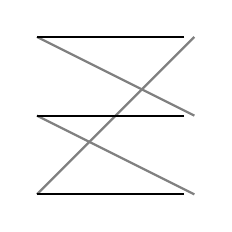
\begin{tikzpicture}[thick,scale=1]

\draw[color = gray] (-1,2)--(1,1);
\draw[color = gray] (-1,1)--(1,0);
\draw[color = gray] (-1,0)--(1,2);

\draw (1, 2) node[]{}
	edge[color = black] (-1, 2);
\draw (-1, 2) node[]{};
\draw (1, 1) node[]{}
	edge[color = black] (-1, 1);
\draw (-1, 1) node[]{};
\draw (1, 0) node[]{}
	edge[color = black] (-1, 0);
\draw (-1, 0) node[]{};


\end{tikzpicture}
	\end{center}
	\caption{A connected matching that is not an ordered connected matching.}
	\label{c_6}
\end{figure}
%
Not every bipartite connected matching is an ordered connected matching, as we see in Figure \ref{c_6}. 
%
 However, it is worth noting that this example is a cycle on six vertices.  
%

Secondly, we define a family of graphs with perfect connected matchings.  Let $L_n$ be a balanced bipartite graph with $2n$ vertices in sets $A = \{a_1, a_2, \ldots, a_3\}$ and $B = \{b_1, b_2, \ldots, b_n\}$.  Each vertex $a_i$ in $A$ is adjacent to precisely those vertices in $B$ whose indices are less than or equal to $i$.  Then then edges between vertices with equal indices form an ordered connected matching.  In Figure \ref{l5} we see an illustration of $L_5$.
\begin{figure}
	\begin{center}
	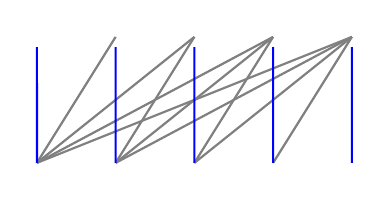
\begin{tikzpicture}[thick,scale=0.8]

%\draw (0, 4) node[words]{$M$};


\draw (3.5, 1) node[]{}
	edge[color = blue] (3.5,-1);
	\draw[color = gray](3.5, 1)-- (2.25,-1);
	\draw[color = gray](3.5, 1)-- (1,-1);
	\draw[color = gray](3.5, 1)-- (-.25,-1);
	\draw[color = gray](3.5, 1)-- (-1.5,-1);
\draw (3.5,-1) node[]{};
\draw (2.25, 1) node[]{}
	edge[color = blue] (2.25, -1);
	
	\draw[color = gray](2.25, 1)-- (1,-1);
	\draw[color = gray](2.25, 1)-- (-.25,-1);
	\draw[color = gray](2.25, 1)-- (-1.5,-1);
\draw (2.25, -1) node[]{};

\draw (1, 1) node[]{}
	edge[color = blue] (1, -1);
	\draw[color = gray](1, 1)-- (-.25,-1);
	\draw[color = gray](1, 1)-- (-1.5,-1);
\draw (1, -1) node[]{};
\draw (-.25,1) node[]{}
	edge[color = blue] (-.25, -1);
	\draw[color = gray](-.25, 1)-- (-1.5,-1);
\draw (-.25, -1) node[]{};

\draw (-1.5,1) node[]{}
	edge[color = blue] (-1.5, -1);
\draw (-1.5, -1) node[]{};

\end{tikzpicture}
	\end{center}
	\caption{The graph $L_5$.}
	\label{l5}
\end{figure} 

Now we consider a hypergraph $H = \{V(H), E(H)\}$.  Let $S = \{S_i\}_{i=1}^k$ be a sequence of subsets of $V(H)$. If for each $i \leq k$ there is a distinct $E_i \in E(H)$ such that $S_i \subseteq E_i$, then we say that $S$ is {\it dominated} by $H$. 
A {\it chain} is a sequence of sets $C_1, C_2, \ldots, C_k$ with the property that $C_i \subsetneq C_{i+1}$ for $1 \leq i <k$.  In this section, we are interested in dominated chains in hypergraphs.

Finally, consider the following computational question:
\begin{framed}\noindent\textbf{Maximum Red Matching Free of Blue-Red Alternating Cycles (MR)}
	\vskip 0.5cm
	\noindent Given a complete bipartite graph $H = (X,Y; E)$ whose edges are partitioned into a set $B$ of blue edges and a set $R$ of red edges and whose vertices are covered by blue edges, what is a maximum matching $M$ in the red component $(X\cup Y, R)$ such that the subgraph $(X,Y; B \cup M)$ has no blue-red alternatiing cycles?
	
\end{framed}

The main result of this section is an equivalence theorem that provides many different perspectives on connected matchings in chordal bipartite graphs.   Before we state the theorem, we need to introduce two ideas.  The first is the {\it biadjacency matrix} $M_B$ of a bipartite graph $G = (A,B;E)$.  This is the (0,1)-matrix formed by indexing rows with the vertices in $A$ and indexing columns with the vertices in $B$.  The element $a_{ij}$ of $M_B$ is 1 if the $ith$ vertex of $A$ is adjacent to the $jth$ vertex of $B$, and zero otherwise.

The second notion we need to introduce is the {\it neigborhood hypergraph} generated by a set $S$ of vertices from a graph $G$.  This is a hypergraph defined on the vertices of $G$ with an edge defined by the open neighborhood of each vertex from $S$.

\begin{theorem}
Let $G= (A,B; E)$ be a chordal bipartite graph.  The following statements are equivalent:
\begin{enumerate}
	\item $G$ has a connected matching of size $k$.
	\item $G$ has an ordered connected matching of size $k$.
	\item $G$ has a copy of $L_k$ as a subgraph.
	\item Tthe neighborhood hypergraph of $A$ has a dominated chain of size $k$.
	\item The biadjacency matrix $M_B$ of the complement $\overline{G}$ of $G$ has a submatrix that is permutation-equivalent to a strictly upper triangular matrix.
	\item For a red/blue edge-colored bigraph $H = (X,Y;B\cup R)$, if $G$ is the red graph $H$, then there is a matching $M$ of size $k$ in $G$ with no alternating blue/red cycle in $(X,Y;B\cup M)$.
\end{enumerate}
\end{theorem}

\begin{proof}
%
First we show that statement 1 is equivalent to statement 2.  We wish to prove that any connected matching $M$ in a chordal bipartite graph $G = (A,B; E)$ has a vertex $a \in A$ so that $a$ is covered by $M$ and $a$ is adjacent to the $B$-endpoints of every edge of $M$.  
%
We say that such a vertex {\it dominates} $M$.  
%
If this is true, we can find the proper ordering of $M$ by sequentially removing the $M$-edge covering a dominating edge and working on the smaller connected matching that remains.

We proceed by induction on the size $n$ of the connected matching.  
%
Small cases of $n = 1,2$ are trivial, and the case of $n=3$ is easily checked.  
%
Now suppose that every chordal bipartite connected matching of up to $n-1$ edges has a dominating vertex and let $M$ be a connected matching of size $n$ in a chordal bipartite graph $G = (A,B;E)$.  
%
Let $H$ be the subgraph of $G$ induced by vertices covered by $M$.
%
Applying lemma \ref{cbp_lemma}, we may remove any bisimplicial edges of $H$ that are not contained in $M$ without reducing the size of $M$; neither does this introduce any new dominating vertices.  
%
Remove these edges until all remaining bisimplicial edges are contained in $M$.  

The resulting graph is chordal bipartite, so there exists a bisimplicial edge $ab \in M$, with $a \in A$ and $b \in B$.  
%
If $a$ is not a dominating vertex, then consider $M_b$, the connected matching contained in $M$ that touches the neighbors of $b$ excluding $a$.  
%
%ADD ILLUSTRATION.  
%
Some $a' \in A$ dominates $M_b$, which means that $a'$ is adjacent to all non-neighbors of $a$.  
%
Furthermore, because the edge $ab$is bisimplicial, $a'$ is adjacent to all of the {\it neighbors} of $a$ as well.  
%
 Hence, $a'$ is a vertex that dominates $M$.  

 We have already noted that $L_k$ contains a connected matching of size $k$. Hence we show now that the subgraph induced by the vertices covered by an ordered connected matching has $L_k$ as a subgraph. This is enough to prove that statement 2 is equivalent to statement 3.
%
 Given an ordered connected matching of size $k$ in a bipartite graph $G$, with a labeling and edge ordering $\sigma$ consistent with the definition of an ordered connected matching, relabel the vertices so that the endpoints of $e_i$ are $a_{\sigma(e_i)}$ and $b_{\sigma(e_i)}$.  Applying the neighborhood inclusion property of ordered connected matchings, it is easy to see that the vertices as labeled induce all the edges of $L_k$.

To show that statement 3 is equivalent to statement 4, let us consider the vertices of $A$ included in the copy of $L_k$ and their neighborhoods within $L_k$.  These form the chain that is dominated by the neighborhoods of these vertices in $G$.  

The complement of our copy of $L_k$ gives us the submatrix of $M_B$ that must be permutation-equivalent to a strictly upper triangular matrix.  By the definition of $L_k$, there is a dominating vertex, and a sequence of vertices wherein each is nonadjacent to at most one more vertex than the last.  By permuting the columns so that the row corresponding to the high degree (in $G$) vertex is at the bottom, and the rows going up correspond to the sequence we just described, we end up with a strictly upper triangular matrix.   

We prove the equivalence of the MR problem to the connected matching problem in chordal bipartite graphs as follows.  First, if there are no alternating blue/red four cycles in $(X, Y; B\cup M)$, then $M$ is certainly a connected matching (in the red graph).  Conversely, consider the copy of $L_k$ contained in a $k$-connected matching.  Any alternating cycle must avoid the ``outer'' edges, and the endpoints of those edges.  Working inductively after removing those edges and vertices, we see that we have a new pair of ``outer'' edges that must be avoided.  Hence, no alternating cycle is present.
\end{proof}

\subsection{Convex graphs}

The {\it convex} graphs are chordal bipartite graphs for which there is a vertex ordering of one side with the property that the neighborhoods of the other side form a collection of intervals.  In this section, we will discuss an attempt at building an algorithm for finding maximum connected matchings in convex graphs that is best described in the language of hypergraphs.
%

Convex graphs can naturally be thought of as the bipartite graph representation of an interval hypergraph.   
%
As such, we inquire after connected matchings in convex graphs by considering the $k$-dominated chain problem for interval hypergraphs.
%
\bprop{The largest set in a chain dominated by an interval hypergraph $H$ can be chosen to be an interval in the ordering of $V(H)$ derived from the interval representation of $H$.}
This is obviously true as all sets in the chain are subsets of the interval dominating the top element in the chain.  Due to this fact, and the fact that there are only polynomially many subintervals of a finite interval, it  suffices to find a polynomial-time algorithm for the problem of finding a {\it perfect} dominated chain in interval hypergraphs.  If this is possible, we need only check every interval for a perfect chain dominated by $H$.
\begin{framed}\noindent\textbf{Dominated k-chain}
	\vskip 0.5cm
	\noindent Input: Hypergraph $H$, positive integer $k$
	
	\noindent Question: Is there a chain of length $k$ dominated by $H$?
\end{framed}

Let $H$ be an interval hypergraph.  We call the intersection of all intervals $C = \bigcap_{e \in E(H)} e$ in an interval hypergraph the {\it cap} of the hypergraph.  
%
We are especially interested in two collections of intervals, $R = \{I \in H : I \geq C\}$, and $L = \{I \in H : I \leq C\}$.
%
\begin{figure}
	\begin{center}
	\begin{tikzpicture}[thick,scale=0.8]

	\coordinate (a1) at (0,1);
	\coordinate (b1) at (1,1); 
	\coordinate (c1) at (2,1);
	\coordinate (d1) at (3,1);
	\coordinate (e1) at (4,1);
	\coordinate (f1) at (5,1);
	\coordinate (g1) at (6,1);

	\coordinate (a2) at (0,2);
	\coordinate (b2) at (1,2); 
	\coordinate (c2) at (2,2);
	\coordinate (d2) at (3,2);
	\coordinate (e2) at (4,2);
	\coordinate (f2) at (5,2);
	\coordinate (g2) at (6,2);

	\coordinate (a3) at (0,3);
	\coordinate (b3) at (1,3); 
	\coordinate (c3) at (2,3);
	\coordinate (d3) at (3,3);
	\coordinate (e3) at (4,3);
	\coordinate (f3) at (5,3);
	\coordinate (g3) at (6,3);

	\coordinate (a4) at (0,4);
	\coordinate (b4) at (1,4); 
	\coordinate (c4) at (2,4);
	\coordinate (d4) at (3,4);
	\coordinate (e4) at (4,4);
	\coordinate (f4) at (5,4);
	\coordinate (g4) at (6,4);

	\coordinate (a5) at (0,5);
	\coordinate (b5) at (1,5); 
	\coordinate (c5) at (2,5);
	\coordinate (d5) at (3,5);
	\coordinate (e5) at (4,5);
	\coordinate (f5) at (5,5);
	\coordinate (g5) at (6,5);

	\coordinate (a6) at (0,6);
	\coordinate (b6) at (1,6); 
	\coordinate (c6) at (2,6);
	\coordinate (d6) at (3,6);
	\coordinate (e6) at (4,6);
	\coordinate (f6) at (5,6);
	\coordinate (g6) at (6,6);

	\coordinate (a7) at (0,7);
	\coordinate (b7) at (1,7); 
	\coordinate (c7) at (2,7);
	\coordinate (d7) at (3,7);
	\coordinate (e7) at (4,7);
	\coordinate (f7) at (5,7);
	\coordinate (g7) at (6,7);

\draw (a1) node[words]{$v_1$};
\draw (a2) node[words]{$v_1$};
\draw (a3) node[words]{$v_1$};
\draw (a4) node[words]{$v_1$};
\draw (a5) node[words]{$v_1$};
\draw (a6) node[words]{$v_1$};
\draw (a7) node[words]{$v_1$};

\draw (b1) node[words]{$v_2$};
\draw (b2) node[words]{$v_2$};
\draw (b3) node[words]{$v_2$};
\draw (b4) node[words]{$v_2$};
\draw (b5) node[words]{$v_2$};
\draw (b6) node[words]{$v_2$};
\draw (b7) node[words]{$v_2$};

\draw (c1) node[words]{$v_3$};
\draw (c2) node[words]{$v_3$};
\draw (c3) node[words]{$v_3$};
\draw (c4) node[words]{$v_3$};
\draw (c5) node[words]{$v_3$};
\draw (c6) node[words]{$v_3$};
\draw (c7) node[words]{$v_3$};

\draw (d1) node[words]{$v_4$};
\draw (d2) node[words]{$v_4$};
\draw (d3) node[words]{$v_4$};
\draw (d4) node[words]{$v_4$};
\draw (d5) node[words]{$v_4$};
\draw (d6) node[words]{$v_4$};
\draw (d7) node[words]{$v_4$};

\draw (e1) node[words]{$v_5$};
\draw (e2) node[words]{$v_5$};
\draw (e3) node[words]{$v_5$};
\draw (e4) node[words]{$v_5$};
\draw (e5) node[words]{$v_5$};
\draw (e6) node[words]{$v_5$};
\draw (e7) node[words]{$v_5$};

\draw (f1) node[words]{$v_6$};
\draw (f2) node[words]{$v_6$};
\draw (f3) node[words]{$v_6$};
\draw (f4) node[words]{$v_6$};
\draw (f5) node[words]{$v_6$};
\draw (f6) node[words]{$v_6$};
\draw (f7) node[words]{$v_6$};

\draw (1.75, 7.25) -- (3.25, 7.25) -- (3.25, 6.75) -- (1.75, 6.75) -- (1.75, 7.25);
\draw (0.75, 6.25) -- (3.25, 6.25) -- (3.25, 5.75) -- (0.75, 5.75) -- (0.75, 6.25);
\draw (-0.25, 5.25) -- (3.25, 5.25) -- (3.25, 4.75) -- (-0.25, 4.75) -- (-0.25, 5.25);
\draw (1.75, 4.25) -- (5.25, 4.25) -- (5.25, 3.75) -- (1.75, 3.75) -- (1.75, 4.25);
\draw (1.75, 3.25) -- (5.25, 3.25) -- (5.25, 2.75) -- (1.75, 2.75) -- (1.75, 3.25);
\draw (0.75, 2.25) -- (4.25, 2.25) -- (4.25, 1.75) -- (0.75, 1.75) -- (0.75, 2.25);
\draw (-0.25, 1.25) -- (5.25, 1.25) -- (5.25, 0.75) -- (-0.25, 0.75) -- (-0.25, 1.25);

\draw (-1,6)--(-2.5,5.5)--(-1,5);
\draw (6,4)--(7.5,3.5)--(6,3);
\draw (-3,5.5) node[words]{$L$};
\draw (8, 3.5) node[words]{$R$};
\end{tikzpicture}

	\end{center}
	\caption{Diagram of an interval hypergraph.  The cap is $\{v_3,v_4\}$.}
	\label{interval_diag}
\end{figure}
 As in Figure \ref{interval_diag}, we think of these as the intervals that extend only to the left or right (respectively) of the cap.

Let us index the vertices of $H$ $v_1, v_2,...v_k$ according to an interval ordering, reading left to right.
%
Suppose there is a chain $C_1, C_2, \ldots, C_k$ on $V(H)$ that is dominated by $H$.  
%
It must be the case that $C_1$ is a singleton, $C_k = V(H)$, and $|C_i| = |C_{i-1}| + 1$.  
%
Define a permutation $\sigma : [k] \rightarrow [k]$ so that 
\[\sigma(i) = j \:\makebox{ when $v_i \in C_j$ and $v_i \notin C_{j-1}$}.\]
%
In other words, $v_i$ is ``added'' at the $\sigma(i)$th step in the chain.
%
Our chain is completely determined by $\sigma$.
%
To dominate the chain, we suppose that there exists an indexing $E_1, E_2, \ldots, E_k$ of the edges of $H$ so that 
\[\{v_i : \sigma(i) \leq j\} \subseteq E_j\]
%
 We construct an algorithm that chooses vertices to add to the chain together with dominating intervals in a ``step-by-step'' manner.
%
It will be easy to see that if the algorithm succeeds, its output must be a dominated perfect chain.
%

First, note that if $j > i$, and $E_j \subseteq E_i$, then the edge sequence with $E_i$ and $E_j$ interchanged still dominates the chain. 
%
That is, we can take an interval ``too soon'', so long as the interval is contained in the interval it is replacing. 
%
After interchanging the two intervals in the edge sequence, the vertex order $\sigma$ is still intact and corresponds to the dominated chain. 

Our algorithm proceeds by sequentially removing edges and vertices.  Start with all of $H$, and attempt to choose a vertex contained in all $k$  edges of $H$ along with one of the edges of $H$ to be designated $v_1$ and $E_1$.  
%
Then remove this edge and this vertex and do the same for the resulting hypergraph.    
%
If we can proceed until all edges and vertices have been chosen without encountering a hypergraph whose cap is empty, then clearly we have exhibited a perfect chain dominated by $H$.
%
To complete an algorithm for efficiently finding a perfect dominated chain, we must make these choices in such a way that no perfect dominated chains are missed.  As of this writing, we have not been able to describe such a method.  Nonetheless, the following method avoids many of the pitfalls encountered in our search, and is a reasonable place to begin any further attempts.


We first claim that we can choose any vertex of $C$ to be $v_1$.  
%
Suppose $u \in C$ is not $v_1$.  
%
Because $u$ is in every edge of $H$, it can act as the first chain element.  
%
We then move $v_1$ to the place in the sequence of chose vertices formerly occupied by $u$ without disturbing the chain.  
%
Thus, the first step in our algorithm is

\begin{framed}{\bf Step 0.} {\it Choose any element of $C$ to be $v_1$.}
\end{framed}

The problem remains to select an edge of $H$ to dominate $v_1$.  
%
By our earlier observation concerning edges that contain ``later'' edges, if $C \in E(H)$ then we can certainly choose $C$.  So we suppose that $C \notin E(H)$.
%

\begin{framed}{\bf Step 1.}  {\it If $C \in E(H)$, let $E_1$ = $C$.}
\end{framed}

Looking ahead,  we see that we must choose all of $R$ or $L$ before $C$ is exhausted.  
%
Until all elements of either $R$ or $L$ have been chosen, the mutual intersection of remaining edges is a subset of $C$.  
%
If $C$ is exhausted, then only the empty subset remains and the algorithm terminates.
%

\begin{framed}{\bf Step 2.} {\it If both $R$ and $L$ are smaller than $C$, then there is no dominated perfect chain.}
\end{framed}

One of $R$ or $L$ will be used in its entirety when $C$ is exhausted.  
%
We must ensure that the other collection can be used later.
%  
Subroutine 1 is designed to tell us if this is possible.
%
\begin{framed}
\noindent {\bf Subroutine 1.}

\noindent {\bf Input:} Sequence of vertices $u_l, u_{l-1},\ldots,u_1,v_1,v_2,\ldots,v_k$; Set $R$ of nested intervals all containing $v_1$ and not $u_1$; Set $U$ of intervals containing $v_1$ and $u_1$. 

\begin{enumerate}
	\item Assign $v_1$ to the smallest unassigned $R$ set.
	\item If all $R$ sets have been assigned, return {\bf YES}. 
	\item  If $v_2$ does not exist, return {\bf NO}.
	\item If $v_2$ is not in all sets, reassign $v_1$ to the smallest unassigned $U$ set that contains $v_1$ but not $v_2$.  Return {\bf NO} if no such set exists.
	\item Subtract 1 from the index of all $v$-vertices and go to 2.
\end{enumerate}
\end{framed}

For the next step, send $R$, $V(H)-C$ in order and with all $u$ vertices less than $C$ and all $v$ vertices greater than $C$, and $U = E(H) - (L\cup R)$ as input to Subroutine 1.   Then send $L$ with the vertex order suitably reversed.
%

\begin{framed}{\bf Step 3.} {\it If both $L$ and $R$ return {\bf NO} from Subroutine 1, there is no dominated perfect chain.  If (WLOG) $L$ returns {\bf NO} and $R$ returns {\bf YES}, choose $\min L$ to be $E_1$.}  
\end{framed}

We show that if Subroutine 1 is satisfied for $R$ and $L$, then we are free to choose either direction to build our chain.  For brevity, we lean to the left.

\begin{framed}{\bf Step 4.} {\it If both $L$ and $R$ return {\it YES} from Subroutine 1, choose $\min L$ to be $E_1$.}
\end{framed}

Finally, we iterate the process.

\begin{framed}{\bf Step 5.} {\it Remove $v_1$ and $E_1$ from $H$ and begin at Step 0 with the resulting interval hypergraph.}
\end{framed}

The hole in this algorithm lies in whether or not choosing $L$ instead of $R$ when both are safe will miss a perfect dominated chain.  We have been unable to produce a counterexample or a proof.   